%
%  Chris Thoma
%
\documentclass[12pt,fullpage]{article}
\usepackage{fullpage}
\usepackage{psfrag}                                          % LaTeX graphics tool
\usepackage{pslatex}                                         % avoids the default cmr font
\usepackage{graphicx}                                        % graphics package 
\usepackage{epsfig}                                          % figures
\usepackage{hyperref}
\usepackage{color}

\begin{document}

\noindent
{\bf Inverse Gaussian distribution} (from \color{blue}\url{http://www.math.wm.edu/~leemis/chart/UDR/UDR.html}\color{black})

\noindent
The shorthand $X \sim {\rm inverse\ Gaussian}(\lambda,\, \mu)$ is used to indicate that the
random variable $X$ has the inverse Gaussian distribution with parameters $\lambda$ and $\mu$.
An inverse Gaussian random variable $X$ with parameters $\lambda$ and $\mu$ has probability density function 
$$
f(x) = \sqrt {{\frac {\lambda}{2 \pi \, {x} ^ {3}}}} {\kern 0.08 em e ^ {-{\frac {\lambda( x - \mu) ^ {2}} {2 \kern 0.04 em x \mu ^ 2}}}} \qquad \qquad x>0,
$$
for $\lambda > 0$ and $\mu > 0$. 
The inverse Gaussian distribution can be used to model the lifetime of an object.
It has also been used to describe the motion of pollen particles in water and Brownian motion
(Chhikara and Folks, {\it The Inverse Gaussian Distribution:  Theory, Methodology, and Applications}, Marcel Dekker, 1989).
The probability density function with three parameter settings is illustrated below.
{\begin{figure}[h!]
\begin{center}
\psfrag{lab1}{$\lambda \kern -0.08 em = \kern -0.08 em  1,\, \mu \kern -0.08 em  = \kern -0.08 em  1$}
\psfrag{lab2}{$\lambda \kern -0.08 em  = \kern -0.08 em  3,\, \mu \kern -0.08 em  =  \kern -0.08 em  1$}
\psfrag{lab3}{$\lambda \kern -0.08 em  = \kern -0.08 em  3,\, \mu \kern -0.08 em  = \kern -0.08 em  3$}
\psfrag{labx}{$x$}
\psfrag{labf}{$f(x)$}
\includegraphics[width=3.2in]{InversegaussianPlot.ps}
\end{center}
\end{figure}}\\

The cumulative distribution function, survivor function, hazard function, inverse distribution, and cumulative hazard functions on the support of $X$ are mathematically intractable.
The moment generating function of $X$ is
$$
M(t) = E\left[ e ^ {tX} \right] = e ^ {\lambda / \mu}\left(1 - \sqrt{1 - \frac{2 \kern 0.08 em \mu ^ 2 t} {\lambda}}\right) \qquad \qquad t < \frac{\lambda} {2}.
$$
The characteristic function of $X$ is
$$
\phi(t) = E\left[ e ^ {it X} \right] =  e ^ {\lambda / \mu}\left(1 - \sqrt{1 - \frac{2 \kern 0.08 em \mu ^ 2 i t} {\lambda}}\right) \qquad \qquad t < \frac{\lambda} {2}.
$$
The population mean, variance, skewness, and kurtosis of $X$ are
$$
E[X] = \mu \qquad
V[X] = \frac{\mu ^ {\kern 0.08 em 3}} {\lambda} \qquad
E\left[ \left( \frac{X - \mu}{\sigma} \right) ^ 3 \right] = 3 \sqrt{\frac{\mu}{\lambda}} \qquad
E\left[ \left( \frac{X - \mu} {\sigma} \right) ^ 4 \right] = 3 + \frac{15 \mu}{\lambda}.
$$

\vspace{0.1in}

\noindent
{\bf APPL verification:}
The APPL statements
\begin{verbatim}
X:= InverseGaussianRV(lambda, mu);
CDF(X);
Mean(X);
Variance(X);
Skewness(X);
Kurtosis(X);
MGF(X);
\end{verbatim}
verify the cumulative distribution function, the population mean, variance, skewness, kurtosis,  and moment generating function.

\end{document}
